% !TEX root = ./multilinear.tex
\section{Experiments}
\label{sec:experiments}
The experimental study of the proposed parallel algorithms covers the following topics.

\begin{itemize}
\item
\textbf{Effect of partition size.} We analyze performance with partition size as $N_1$ is varied (Section~\ref{sec:perf-part-size}).

\item
\textbf{Scalability with subgraph size.} We depict the total runtime as subgraph size is increased (Section \ref{sec:perf-subgraph-size}).

\item 
\textbf{Strong scaling.} We show the total runtime as the number of parallel processors is increased, thereby reducing the computing workload per process (Section \ref{sec:perf-strong-scaling}).

\item
\textbf{\ouralgo{} vs. FASCIA.} We present the runtime of our implementation compared to FASCIA (Section~\ref{sec:perf-vsfasci}).

\item
\textbf{Scan Statistics and its applications.} We provide performance results for the parallel scan statistics algorithm and present an application (Section \ref{sec:perf-scan-stat}).

\end{itemize}

\subsection{Experimental Setup}
\subsubsection{Hardware}
Experiments were conducted on Juliet, an Intel Haswell HPC cluster. Up to 32 nodes were used for the evaluation, where each node has 36 cores (2 sockets $\times$ 18 cores each). A node consists of 128GB of main memory and 56Gbps Infiniband interconnect. We also tested on another HPC cluster, Shadowfax-Haswell, where we used 32 nodes each with 32 cores (2 sockets $\times$ 16 cores each). Memory and interconnect of this cluster are similar to those of Juliet.

\subsubsection{Datasets}
We evaluate our algorithms on two large graphs: 1) a social contact network of Miami, commonly used in agent-based simulation studies \cite{barrett2009generation}, and 2) a snapshot of the Orkut social network\footnote{\url{https://snap.stanford.edu/data/com-Orkut.html}}. In addition, we perform experiments in two Erdos-Renyi networks of 1 and 10 million nodes with an expected number of edges of $n\log n$, where $n$ is the number of nodes. A summary of the datasets is provided in Table \ref{table:datasets}.

\begin{table}[ht]
\centering \caption{\small Datasets used in our experiments}
\vspace{-.1in}
\label{table:datasets}
%\resizebox{\columnwidth}{!}{
%\begin{scriptsize}
\begin{tabular}{|l|r|r|}
\hline
\textbf{Dataset}  & \textbf{Nodes ($\times 10^6$)} & \textbf{Edges ($\times 10^6$)} \\
\hline
miami & 2.1 & 51.5\\
\hline
com-Orkut  & 3.1 & 234.3\\
\hline
random-1e6 & 1 & 13.8\\
\hline
random-1e7 & 10 & 161.8\\
\hline
\end{tabular}
%\end{scriptsize}
%}
\end{table}

\begin{figure*}[!htb]
    \centering
    \begin{minipage}{0.32\textwidth}
        \centering        
        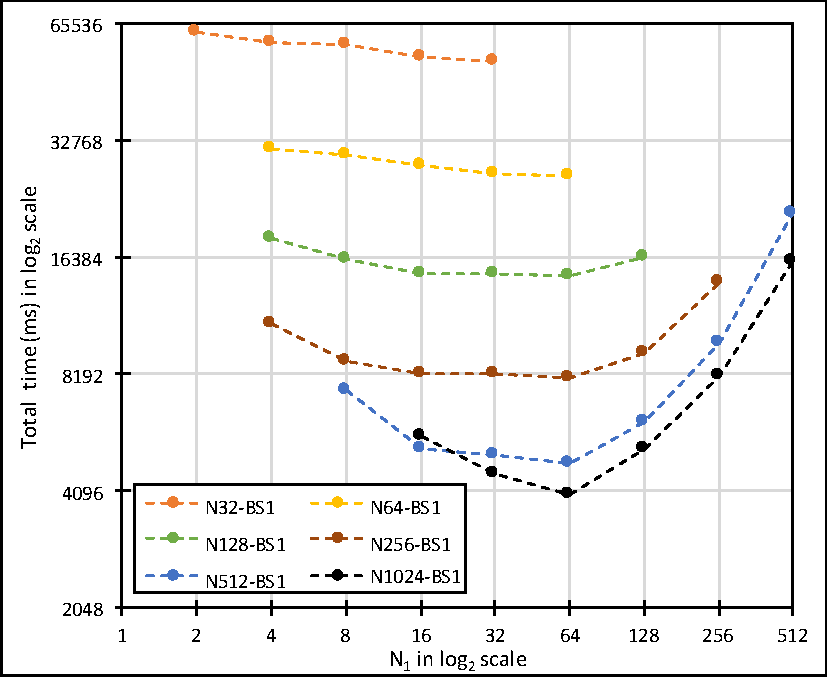
\includegraphics[width=1\columnwidth]{img/kpath-N1N/fig-perf-kpath-1mil-k6-bs1.pdf}
        \caption{$k$-path total runtime for random-1e6 and varying $N_1$. Note. $BS1=N_2=1$}
        \label{fig:fig-perf-kpath-1mil-k6-bs1.pdf}
    \end{minipage}
    \hspace{0mm}
    \begin{minipage}{0.32\textwidth}
        \centering
        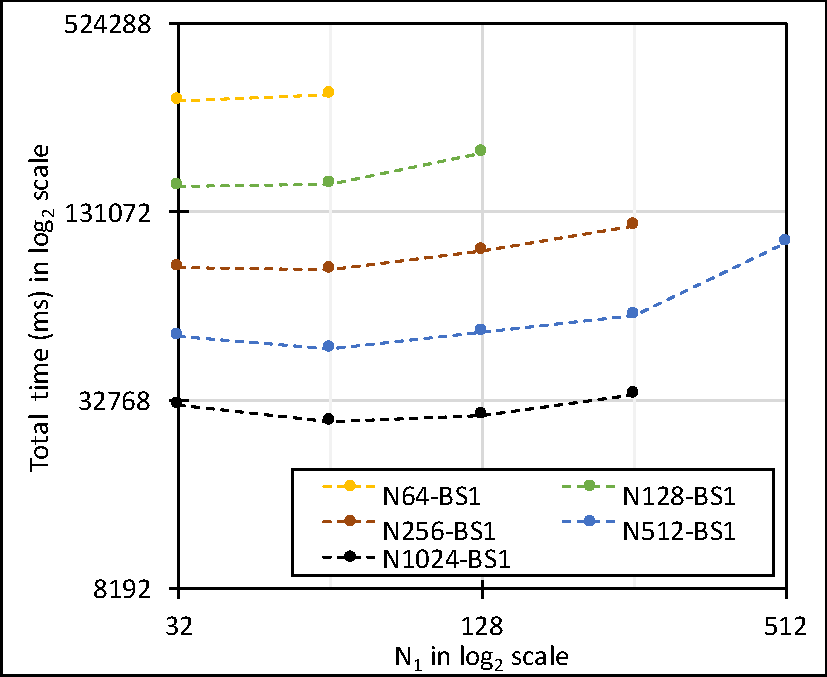
\includegraphics[width=1\columnwidth]{img/kpath-N1N/fig-perf-kpath-orkut-k6-bs1.pdf}
        \caption{$k$-path total runtime for com-Orkut and varying $N_1$. Note. $BS1=N_2=1$}
        \label{fig:fig-perf-kpath-orkut-k6-bs1.pdf}
    \end{minipage}  
    \hspace{0mm}
    \begin{minipage}{0.33\textwidth}
        \centering
        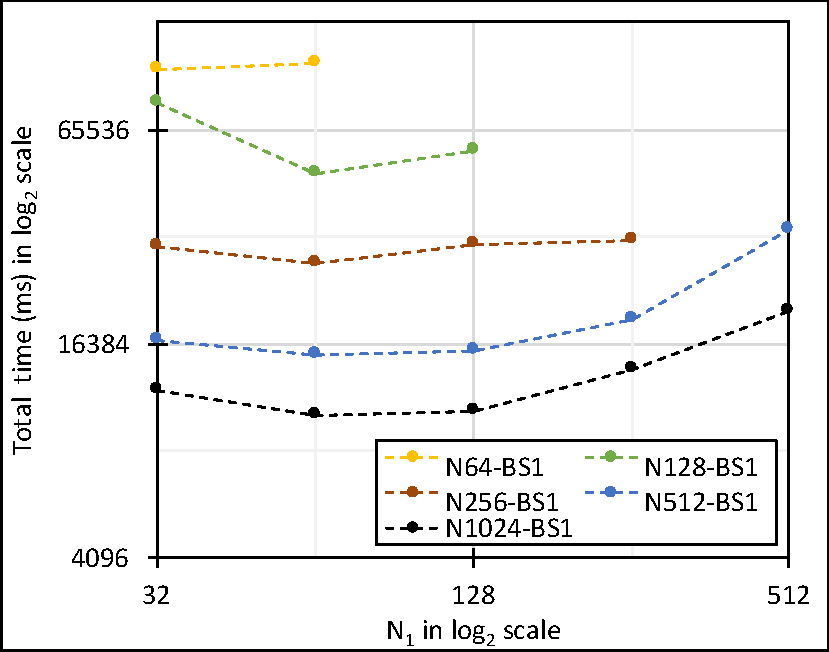
\includegraphics[width=1\columnwidth]{img/kpath-N1N/fig-perf-kpath-miami-k6-bs1.pdf}
        \caption{$k$-path total runtime for miami and varying $N_1$. Note. $BS1=N_2=1$}
        \label{fig:fig-perf-kpath-miami-k6-bs1.pdf}
    \end{minipage}  
\end{figure*}

\begin{figure*}[!htb]
    \centering
    \begin{minipage}{0.32\textwidth}
        \centering        
        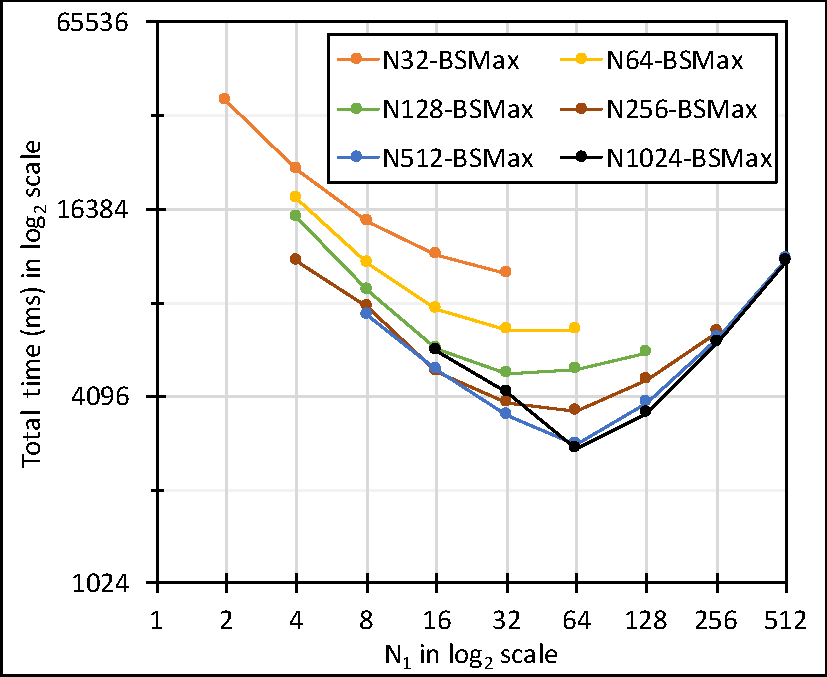
\includegraphics[width=1\columnwidth]{img/kpath-N1N/fig-perf-kpath-1mil-k6-bsmax.pdf}
        \caption{$k$-path total runtime for random-1e6 and varying $N_1$. Note. $BSMax=N_2=2^kN_1/N$}
        \label{fig:fig-perf-kpath-1mil-k6-bsmax.pdf}
    \end{minipage}
    \hspace{0mm}
    \begin{minipage}{0.32\textwidth}
        \centering
        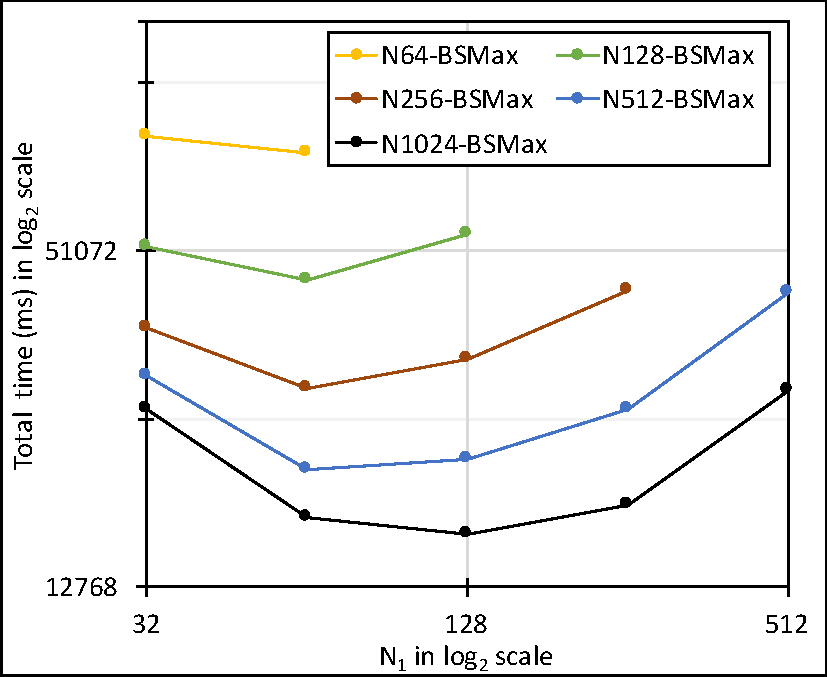
\includegraphics[width=1\columnwidth]{img/kpath-N1N/fig-perf-kpath-orkut-k6-bsmax.pdf}
        \caption{$k$-path total runtime for com-Orkut and varying $N_1$. Note. $BSMax=N_2=2^kN_1/N$}
        \label{fig:fig-perf-kpath-orkut-k6-bsmax.pdf}
    \end{minipage}  
    \hspace{0mm}
    \begin{minipage}{0.32\textwidth}
        \centering
        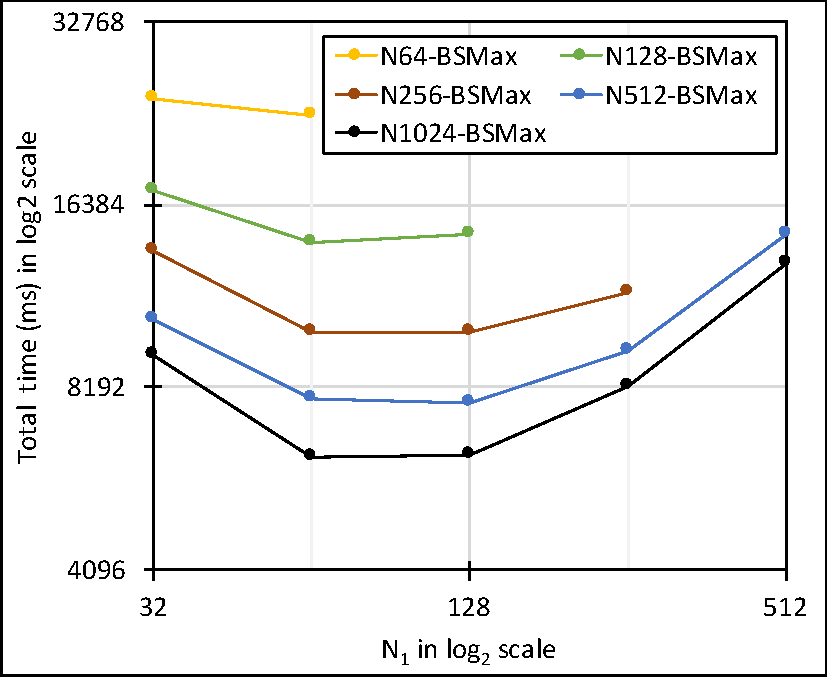
\includegraphics[width=1\columnwidth]{img/kpath-N1N/fig-perf-kpath-miami-k6-bsmax.pdf}
        \caption{$k$-path total runtime for miami and varying $N_1$. Note. $BSMax=N_2=2^kN_1/N$}
        \label{fig:fig-perf-kpath-miami-k6-bsmax.pdf}
    \end{minipage}  
\end{figure*}

% [Saliya] I think we don't need this section on
% independence of iterations because now we don't
% run these as separate instances. Everything is 
% automatically done within the program.
% \subsection{Independence of Iterations}
% \label{sec:independence}
% First, we examine the extent to which the $2^k$ iterations of the outer loop in
% Algorithm \parmaxwt{} are independent and take the same time. Figure \ref{fig:indep} shows the running time as the number of processors $N$ is increased for the random network of 1 million nodes. This figure implies that the running time is almost invariant with the
% number of parallel iterations that are run simultaneously. We observed similar results with com-Orkut graph as shown in Figure~\ref{fig:indep-orkut}. We use this insight to estimate the total running time for other settings. 

% \begin{figure}[!htpb]
% 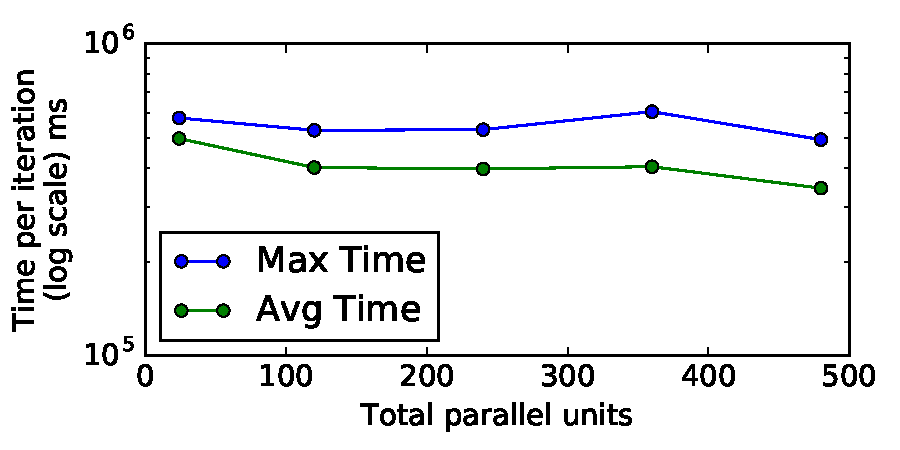
\includegraphics[width=0.4\textwidth]{img/fig-random-1mil-timeperiteration.pdf}
% \caption{Time per iteration with varying parallel units for random 1 million nodes network.}
% \label{fig:indep}
% \end{figure}

% \begin{figure}[!htpb]
% 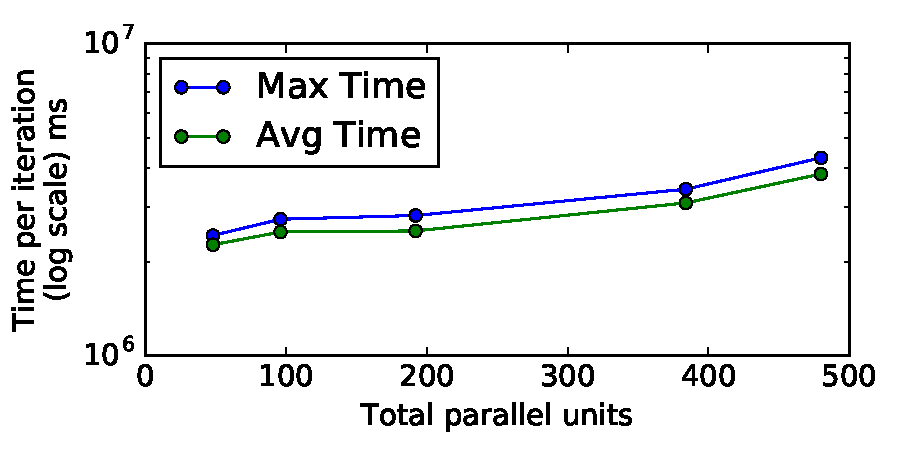
\includegraphics[width=0.4\textwidth]{img/fig-orkut-timeperiteration.pdf}
% \caption{Time per iteration with varying parallel units for Orkut network.}
% \label{fig:indep-orkut}
% \end{figure}

\subsection{Effect of partition size}
\label{sec:perf-part-size}
Our parallel $k$-Path algorithm exhibits two levels of parallelism: vertex and iterations. On one hand, the $2^k$ iterations are pleasingly parallel except for a global reduction at the end. The parallel vertex computation within each iteration, on the other hand, requires message passing between neighbors for $k-1$ steps---in the case of trees, this would be the number of sub-templates instead of $k-1$. 

% \textcolor{blue}{TODO - change bs to N2}

Given these two levels of parallelism and a total of $N$ processes, we can split the $2^k$ iterations among $a=N/N_1$  parallel phases. Each phase decomposes the graph across $N_1$ processes and performs the $k$-Path computation in parallel for $2^k/a$. To reduce the communication over computation cost, the algorithm packs a user defined $N_2$ number of iterations into one computation step, so each parallel phase only has to perform $ 2^k/(a*N_2)$ compute and communication phases. 
To illustrate this with an example, consider the case of $k=6$, $N=128$, $N_1=32$, and $N_2=8$. The total number of iterations is $2^k = 64$. The number of parallel phases corresponding to $N_1=32$ is $128/32 = 4$. Each phase only needs to run $64/4 = 16$ iterations. Since $N_2=8$, the $16$ iterations can be completed in just $16/8 = 2$ batches.

Increasing $N_2$, for example $N_2=16$ in the previous case, would allow us to finish the entire program in one compute and communicate batch. This results in higher parallel efficiency as the overhead of communication to computation is reduced. However, it increases the message size by a factor of $N_2$\footnote{Increasing message size for a communication step is not necessarily bad. Reducing the number of small messages in communication may lead to increased network performance\cite{smallmessagecoalasce}.}. Depending on the number of total processes, MPI may fail to accommodate very large message sizes requiring to reduce $N_2$, so that some form of chunking method may be required. 

%We evaluate the total time to complete for $k$-Path and scan statistics as a function of $N_1$, the number of processes used to run 
%each of the $2^k$ circuit evaluations. Figure \ref{fig:time-with-p} shows the total time for both applications varying $N$ and $N_1$. First, we note that, as $N$ becomes larger, the total running time decreases for all values of $N_1$, which is expected. Second, we obtain the best performance by assigning around 8 parallel units to process an iteration, regardless of the total parallel units.

% Figure 3 and Figure 6 --> As N1 increase message parallalization of compute regions increase, but this also increase number of communication steps. 
% For N2 = 1
Figures~\ref{fig:fig-perf-kpath-1mil-k6-bs1.pdf}, \ref{fig:fig-perf-kpath-orkut-k6-bs1.pdf}, \ref{fig:fig-perf-kpath-miami-k6-bs1.pdf} show the performance of \ouralgo{} on three different datasets when $N_2=1$. We observe that running times of \ouralgo{} when $N_2$ is scaled for a fixed value of $N$ for each problem size---this effectively tested our parallel algorithm for a large range of configurations. Our observations confirm the existence of an optimal point (i.e., a minimum) between the two levels of parallelism discussed before. The communication cost gradually increases when moving from one extreme end of parallelism to the other because of the increase in number of messages exchanged \footnote{Number of messages exchanged can be approximated to $O(\log{N_1})$ for small message sizes where $N_1$ ranges from $N_1=1$ to $N_1\rightarrow N$}. However, at the optimal point, the cost of communication can be sufficiently amortized by the amount of parallelism gained. In other words, the optimal setting for \ouralgo{} can be found in a point between vertex level and iteration based parallelism. 

The observed speedup (1x to 2x) is due to cache affinity effects on the main loop and reduction of communication phases by increasing the message size.
Interestingly, when $N_2$ is increased (Figures~\ref{fig:fig-perf-kpath-1mil-k6-bsmax.pdf}, \ref{fig:fig-perf-kpath-orkut-k6-bsmax.pdf}, \ref{fig:fig-perf-kpath-miami-k6-bsmax.pdf}) we observe further relative performance gains on the same set of experiments. Furthermore, speedups are evident for each experiment instance of the $k$-path problem when problem size is scaled. As a general guideline, we find that keeping $N_1$ close to the number of cores in one or two machines lead to better performance. A more formal characterization of the trade-off between $N_1$ and $N_2$ is a topic for future work.


\begin{figure*}[!htb]
    \centering
    \begin{minipage}{0.29\textwidth}
        \centering        
        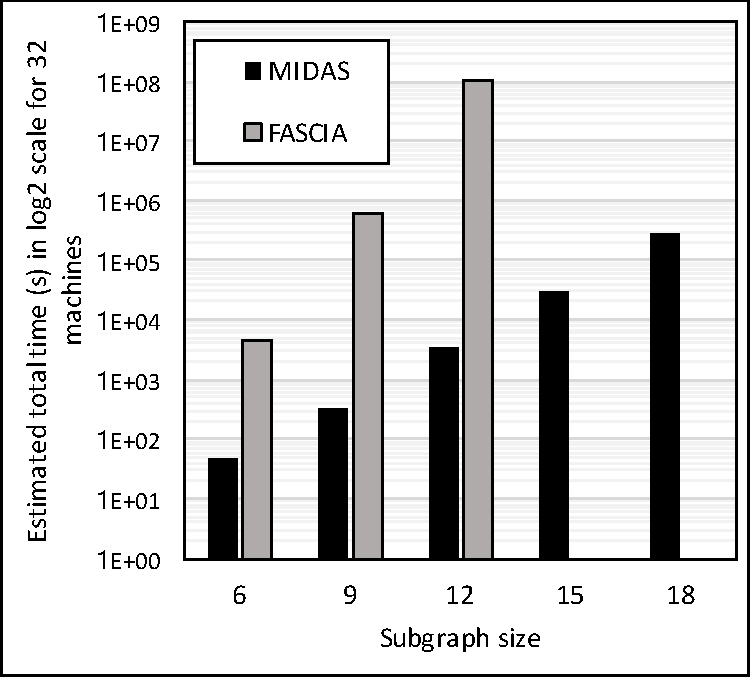
\includegraphics[width=1\columnwidth]{img/fig-perf-vsfascia.pdf}
        \caption{\ouralgo{} runtime compared to FASCIA for varying subgraph sizes in the $k$-path problem}
        \label{fig:fig-perf-vsfascia.pdf}
    \end{minipage}
    \hspace{0mm}
    \begin{minipage}{0.32\textwidth}
        \centering        
        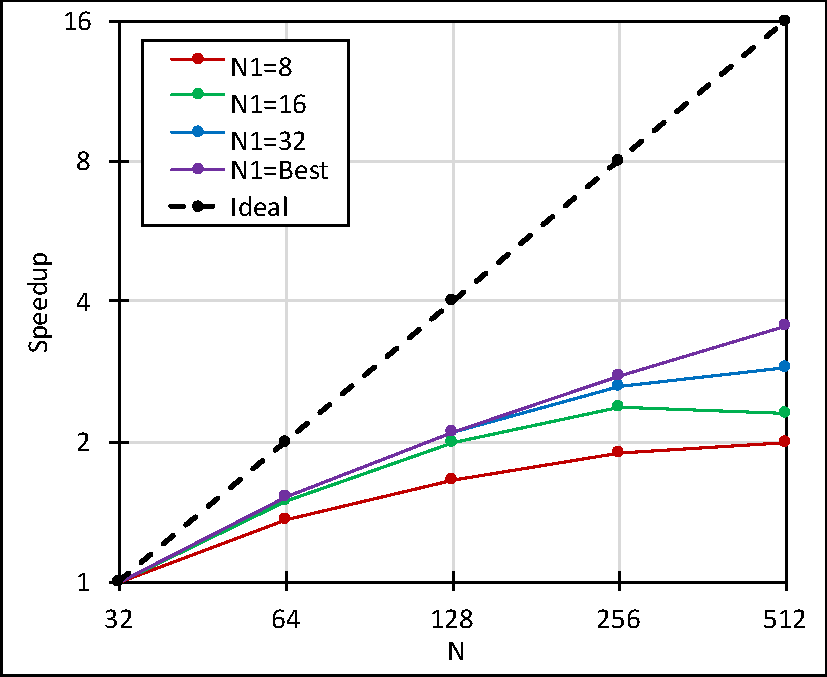
\includegraphics[width=1\columnwidth]{img/kpath-N1N/fig-perf-kpath-1mil-speedup-N1fixed.pdf}
        \caption{\ouralgo{} strong scaling for the $k$-path problem with increasing $N$, while $N_1$ is fixed.}
        \label{fig-perf-kpath-1mil-speedup-N1fixed.pdf}
    \end{minipage}
    \hspace{0mm}
    \begin{minipage}{0.32\textwidth}
        \centering        
        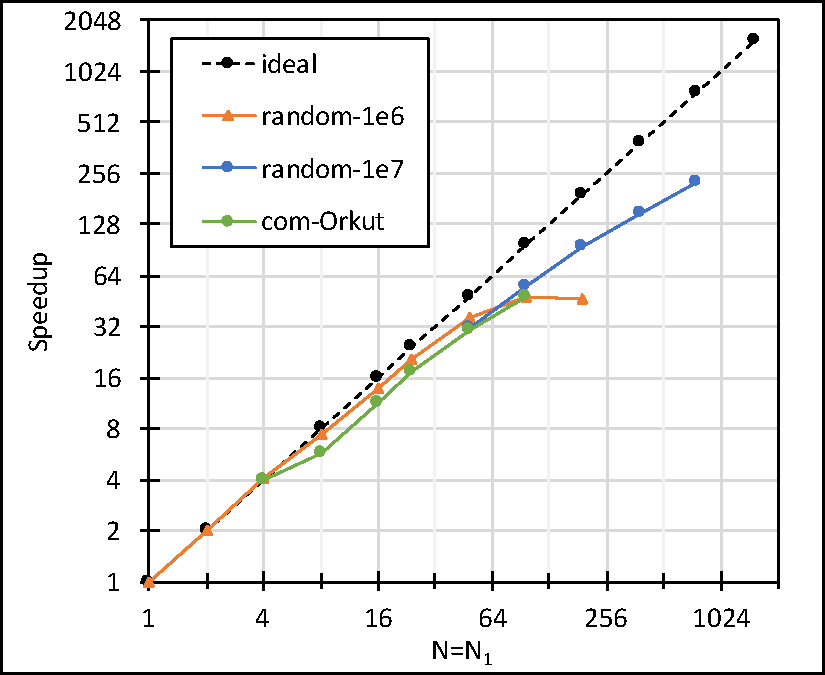
\includegraphics[width=1\columnwidth]{img/kpath-N1N/fig-perf-kpath-speedup-N=N1.pdf}
        \caption{\ouralgo{} strong scaling for the $k$-path problem with increasing $N$ and $N_1=N$}
        \label{fig:fig-perf-kpath-speedup-N=N1.pdf}
    \end{minipage}
\end{figure*}

\begin{figure*}[!htb]
    \centering
    \begin{minipage}{0.32\textwidth}
        \centering        
        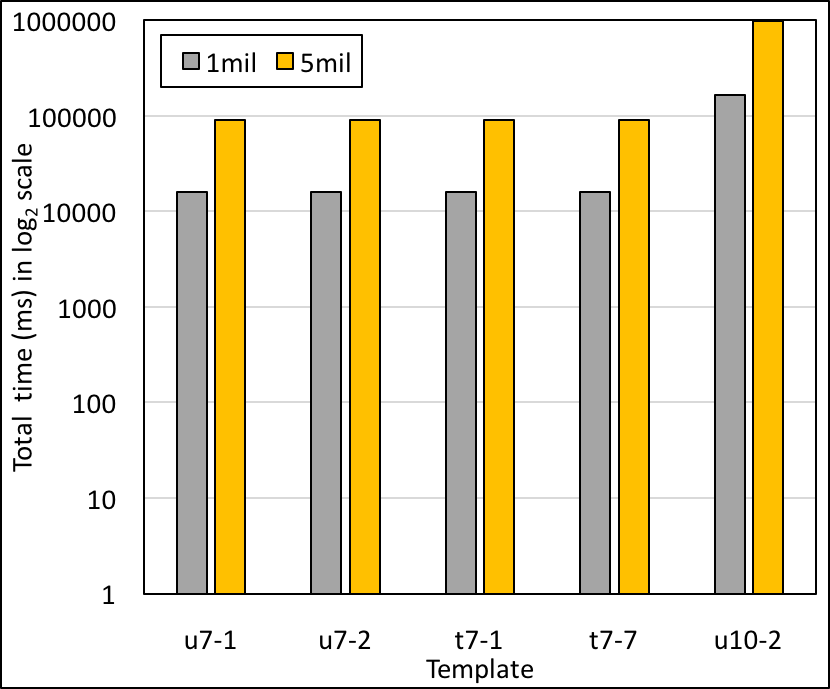
\includegraphics[width=1\columnwidth]{img/ktree/ktree-1mil-5mil-16nodes.png}
        \caption{$k$-tree total runtime for random 1e6 and 5e6 for different templates. Note. $N=16$}
        \label{fig:ktree-1mil-5mil-16nodes.png}
    \end{minipage}
    \hspace{0mm}
    \begin{minipage}{0.32\textwidth}
        \centering        
        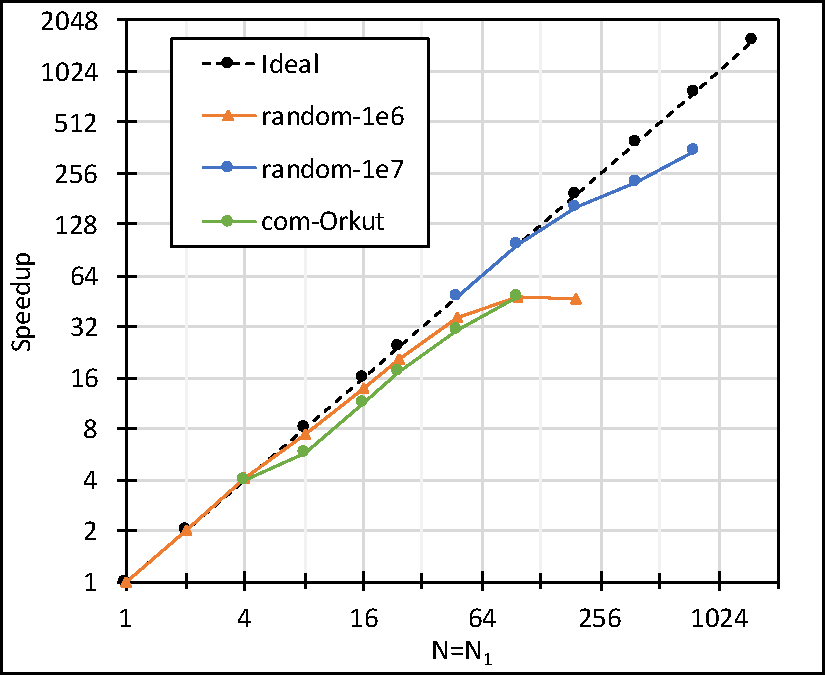
\includegraphics[width=1\textwidth]{img/fig-perf-scan-speedup-N=N1.pdf}
        \caption{\ouralgo{} strong scaling for the scan statistics problem with increasing $N$ and $N_1=N$}
        \label{fig:fig-perf-scan-speedup-N=N1.pdf}
    \end{minipage}  
    \hspace{0mm}
    \begin{minipage}{0.32\textwidth}
        \centering
        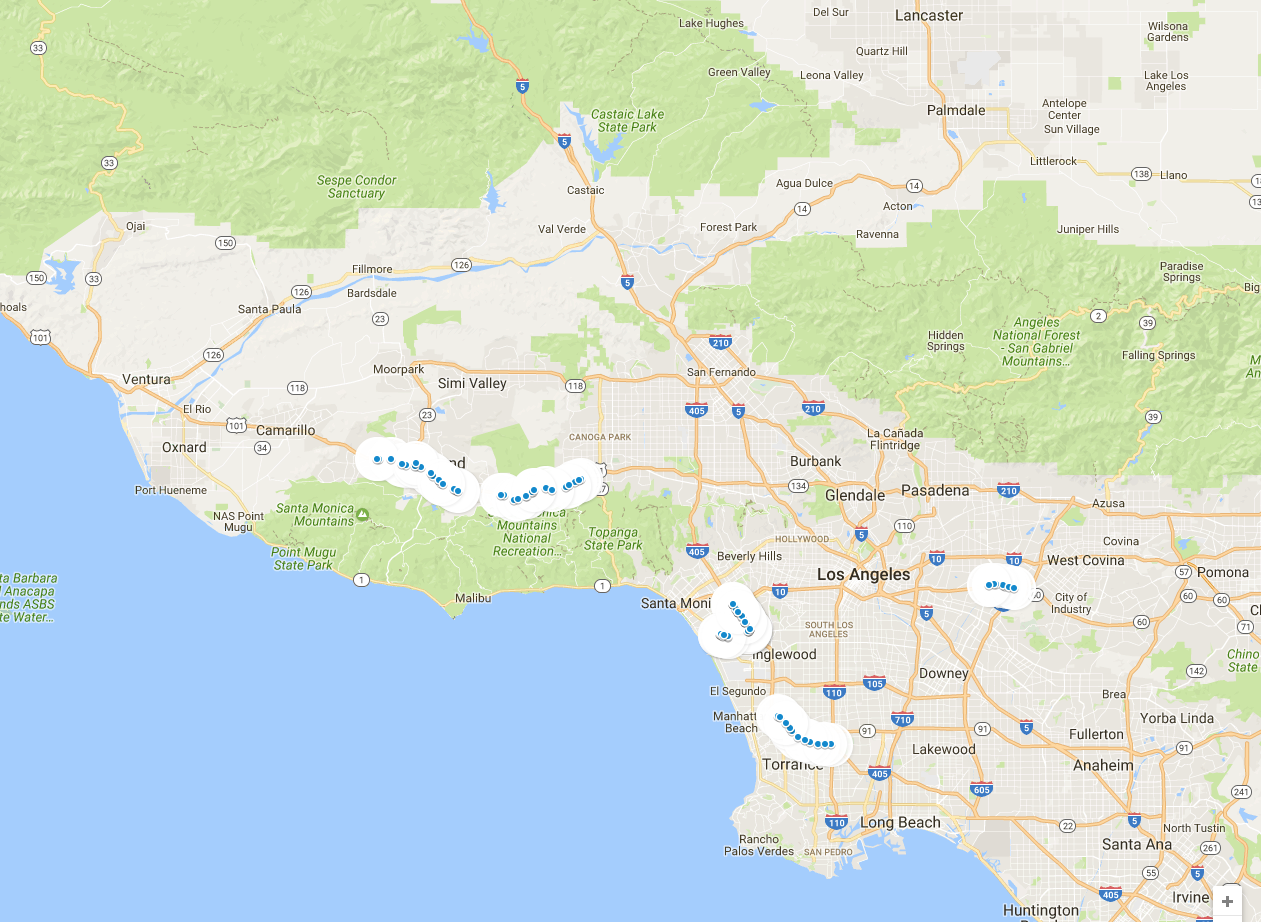
\includegraphics[width=1\textwidth]{img/traffic-example.png}
        \caption{Discovering highway segments with unexpected congestion in the Los Angeles road network.}
        \label{fig:traffic}
    \end{minipage}  
\end{figure*}

% \begin{figure*}[!htb]
%     % \centering
%     \begin{minipage}{0.2\textwidth}
%         \centering        
%         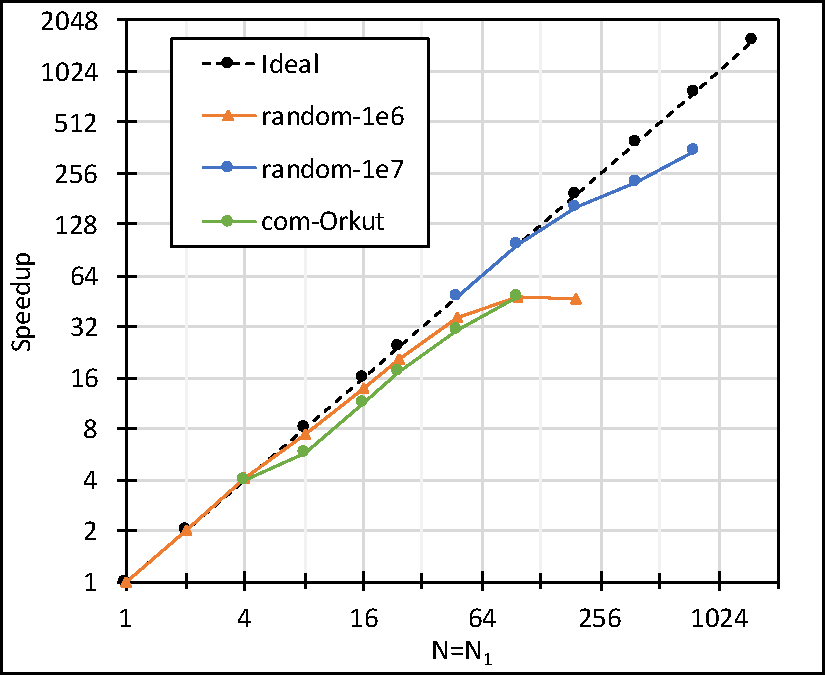
\includegraphics[width=1\columnwidth]{img/fig-perf-scan-speedup-N=N1.pdf}
%         \caption{\ouralgo{} strong scaling for the Scan Statistics problem with increasing $N$ and $N_1=N$}
%         \label{fig:fig-perf-scan-speedup-N=N1.pdf}
%     \end{minipage}
%     \hspace{0mm}
%     \begin{minipage}{0.2\textwidth}
%         \centering
%         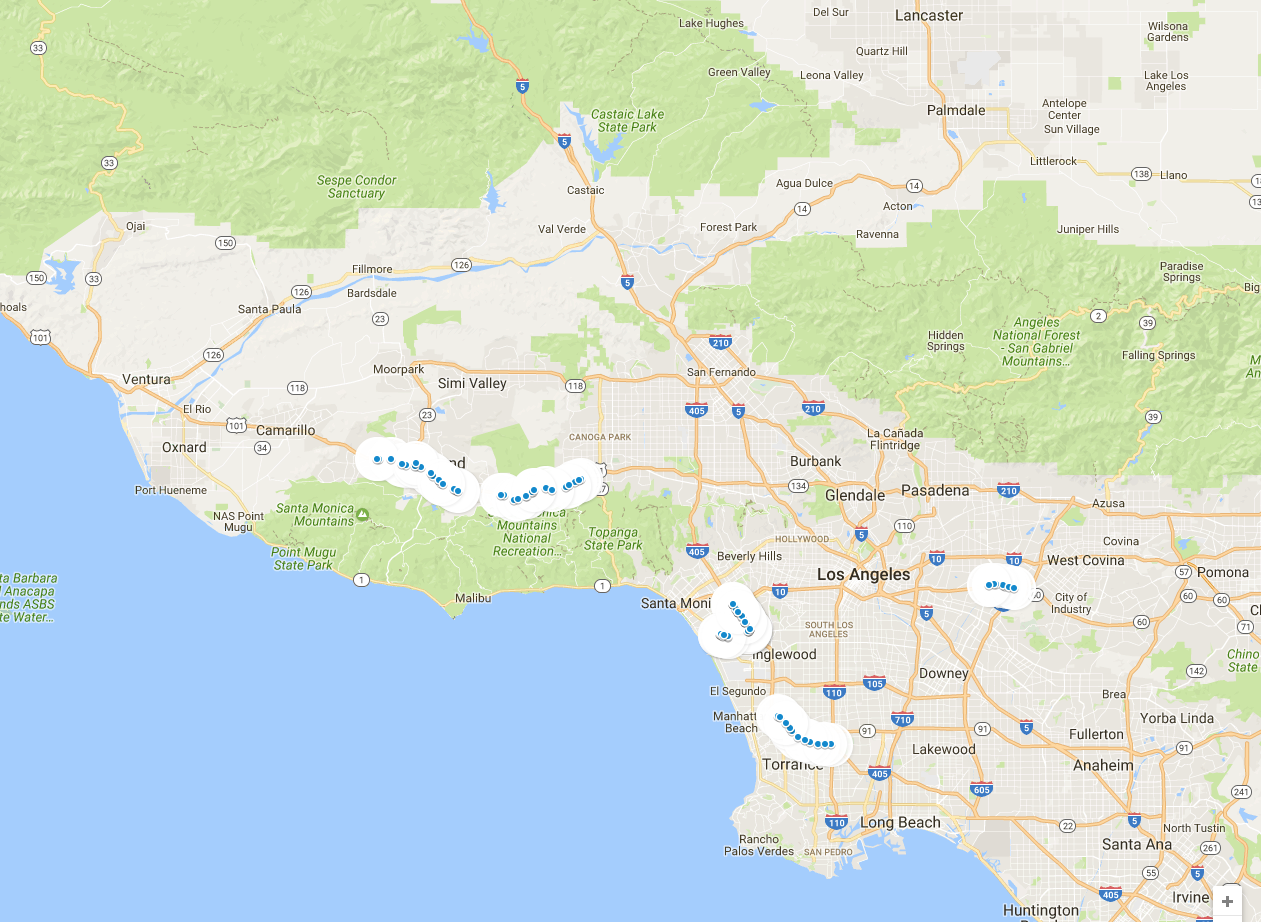
\includegraphics[width=1\columnwidth]{img/traffic-example.png}
%         \caption{Discovering highway segments with unexpected congesion in the Los Angeles road network.}
%         \label{fig:traffic}
%     \end{minipage}
% \end{figure*}

% \begin{figure}
%     \centering        
%     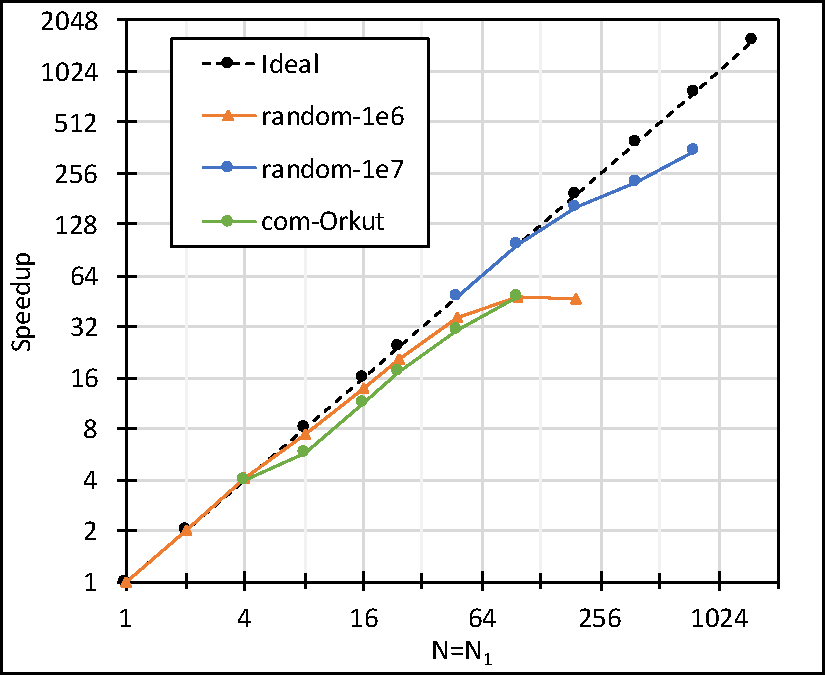
\includegraphics[width=0.6\columnwidth]{img/fig-perf-scan-speedup-N=N1.pdf}
%     \caption{\ouralgo{} strong scaling for the Scan Statistics problem with increasing $N$ and $N_1=N$}
%     \label{fig:fig-perf-scan-speedup-N=N1.pdf}
% \end{figure}

% \begin{figure}
%     \centering
%     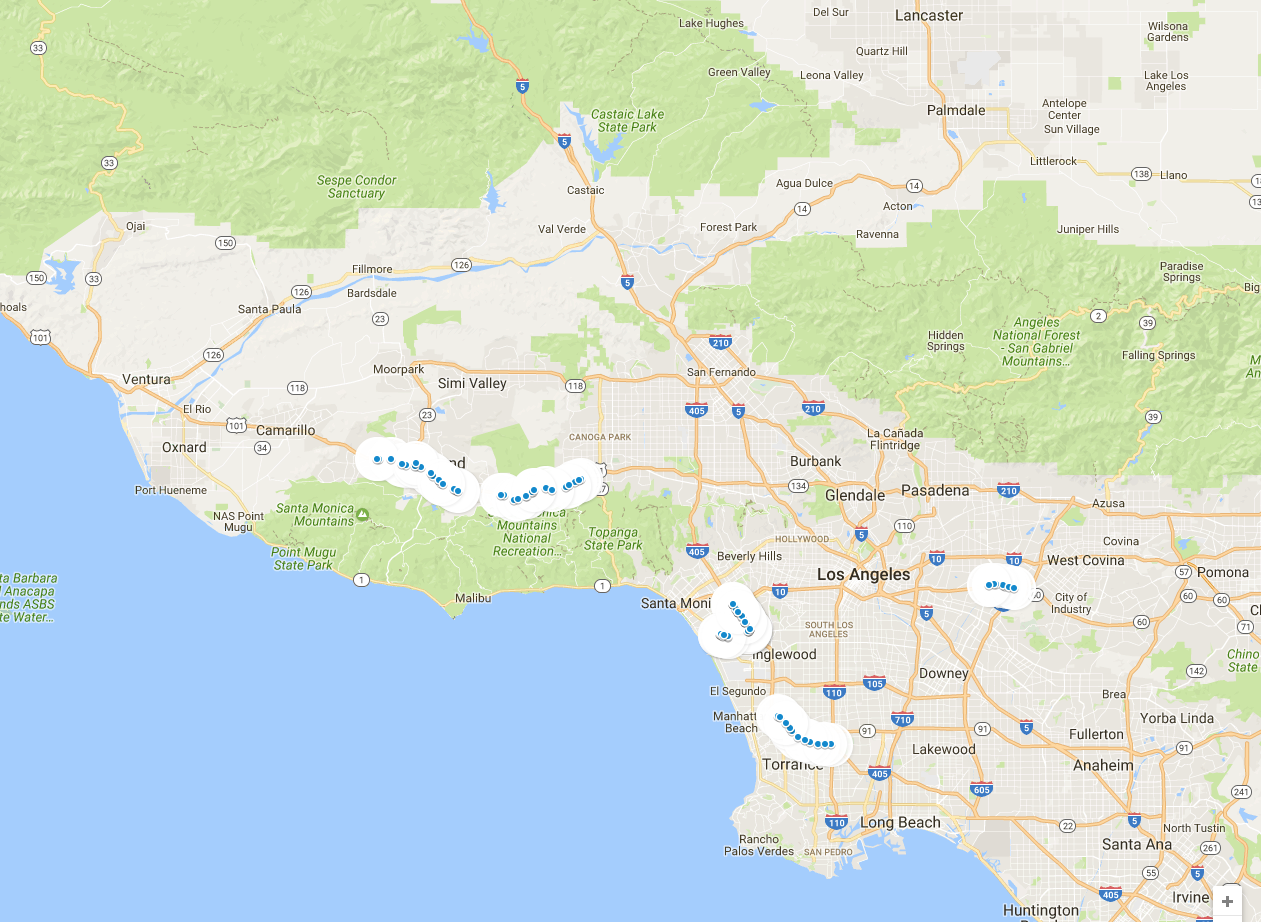
\includegraphics[width=0.6\columnwidth]{img/traffic-example.png}
%     \caption{Discovering highway segments with unexpected congesion in the Los Angeles road network.}
%     \label{fig:traffic}
% \end{figure}


\subsection{Scalability with subgraph size}
\label{sec:perf-subgraph-size}
In Figure~\ref{fig:fig-perf-vsfascia.pdf}, we increase the subgraph size, $k$, in both FASCIA and \ouralgo{}, while keeping $N$ and $N_1$ fixed. Figures~\ref{fig:fig-perf-kpath-1mil-k6-bsmax.pdf}--\ref{fig:fig-perf-kpath-miami-k6-bsmax.pdf} suggest it is best to keep $N_2$ as high as possible to leverage the cache locality benefits discussed above. However, the total message size communicated out of a process increases with $N_2$ leading to diminishing returns. Therefore, we've kept $N_2<1024$. %The results in Figure~\ref{fig:fig-perf-scan-speedup-N=N1.pdf} verifies the total runtime grows exponentially with subgraph size, $k$ in this case.

\subsection{Strong  scaling}
\label{sec:perf-strong-scaling}
The strong scaling of \ouralgo{} can be investigated in two ways. The first is to fix $N_1$ and change $N$, thereby increasing the parallel phases to split the $2^k$ iterations. We could observe the effect of this behavior by examining the values along a fixed $N_1$ value in Figures~\ref{fig:fig-perf-kpath-1mil-k6-bs1.pdf}--\ref{fig:fig-perf-kpath-miami-k6-bsmax.pdf}. Dividing the runtime corresponding to the minimum $N$ (the top most line) by the given $N$ gives speedup indicating the strong scalability of \ouralgo{}. 

Figure~\ref{fig-perf-kpath-1mil-speedup-N1fixed.pdf} presents such speedup for a set of $N_1$ values over varying $N$. We observe the results do not necessarily scale linearly due to the fact that communication within a phase is dominant. We get the best speedup by going along points in Figures~\ref{fig:fig-perf-kpath-1mil-k6-bs1.pdf}--\ref{fig:fig-perf-kpath-miami-k6-bsmax.pdf} that gave the minimum runtime. This is shown as the $N1=\text{Best}$ line in Figure~\ref{fig-perf-kpath-1mil-speedup-N1fixed.pdf}.

The other form of strong scalability we can test is by setting $N1=N$. This produces a single phase and is the classic strong scaling of parallel graph algorithms. Figure~\ref{fig:fig-perf-kpath-speedup-N=N1.pdf} presents the speedup values for different datasets. Even though the speedups are less than ideal, we still observe good performance up to a considerable number of processes.

\subsection{\ouralgo{} vs.\ FASCIA}
\label{sec:perf-vsfasci}
Figure~\ref{fig:fig-perf-vsfascia.pdf} compares the running time of FASCIA to \ouralgo{} for varying subgraph sizes. We see FASCIA fails to support beyond subgraphs of size 12 on the random-1e6 graph, whereas \ouralgo{} scales to well over 18. Also, \ouralgo{} shows a significant improvement over FASCIA in runtime. Figure~\ref{fig:ktree-1mil-5mil-16nodes.png} shows \ouralgo{} performance for different tree templates of random-1e6 and random-5e6. The details of the templates can be found in the FASCIA papers~\cite{slota:icpp13, slota:ipdps14}.

\subsection{Scan statistics optimization}
\label{sec:perf-scan-stat}
In Figure~\ref{fig:fig-perf-scan-speedup-N=N1.pdf}, we present strong scaling results for the scan statistics problem where $N_1$ is set to $N$. We do this for multiple datasets and observe considerable strong scalability similar to the $k$-Path problem in Figure~\ref{fig:fig-perf-kpath-speedup-N=N1.pdf}.

We apply our algorithm for scan statistics to find clusters with unexpectedly low-moving traffic in the highway network of Los Angeles County\footnote{\url{http://pems.dot.ca.gov/}}. Nodes in the graph are sensors next to the road that record the average speed and the number of vehicles passing through. We have 30-minute snapshots for May 2014. We assume that the average speed recorded by each sensor follows a normal distribution. Then, the $p$-value of a node $i$ is the cumulative distribution function of a normal distribution with mean  $\mu_i^{[1,t-1]}$ and standard deviation $\sigma_i^{[1,t-1]}$, where $\mu_i^{[1,t-1]}$ and $\sigma_i^{[1,t-1]}$ are, respectively, the sample mean and standard deviation for node $i$ from snapshots $1$ to $t-1$.

We use our algorithm with $k=12$ on this dataset. In Figure \ref{fig:traffic}, we show with blue dots highway segments that our algorithm identifies as having \emph{unexpectedly} low average speed during rush hour (16:00 to 19:00) on Friday May 9, 2014. These segments are not necessarily the ones with most congestion. For instance, the center of Los Angeles city has higher congestion; however, such activity is normal on Friday afternoons according to the previous snapshots. The clusters shown in the map are selected because they have significantly lower average speeds than in previous observations.  

% \subsection{Strong Scaling and Speedup}
% \label{sec:perf-strong-scaling}
% In Figure \ref{fig:scaling}, we show the speed up and strong scaling achieved by increasing the total parallelism. We obtain higher speed up for $k$-Path, possibly because the communication overhead for this program is lower than for Multilinear Scan. In both cases, we the scaling factor is better for the LiveJournal network.

% \begin{figure*}[ht]
%   \centering
%   \begin{subfigure}[b]{\textwidth}
%     \centering
%     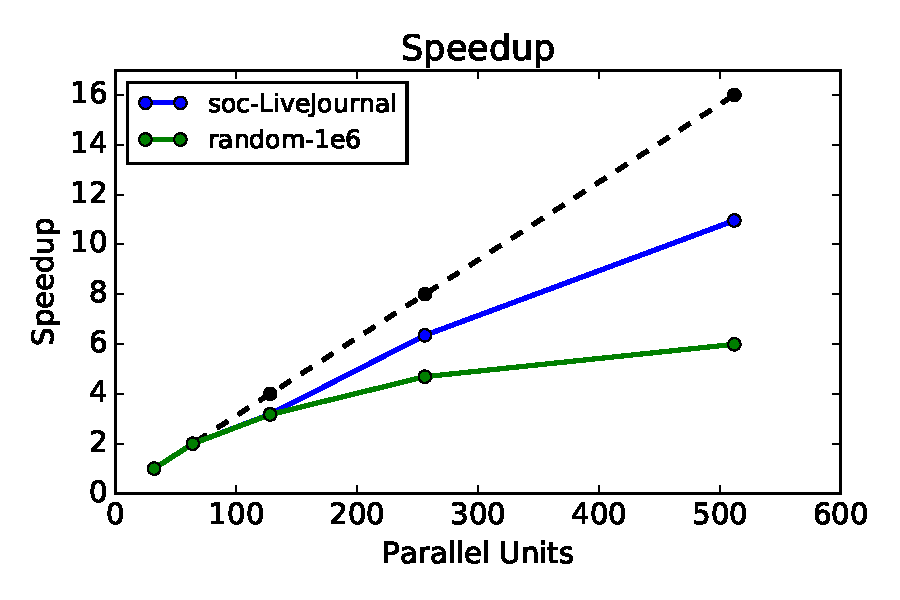
\includegraphics[width=0.45\textwidth]{img/speedup-kpath.pdf}
%     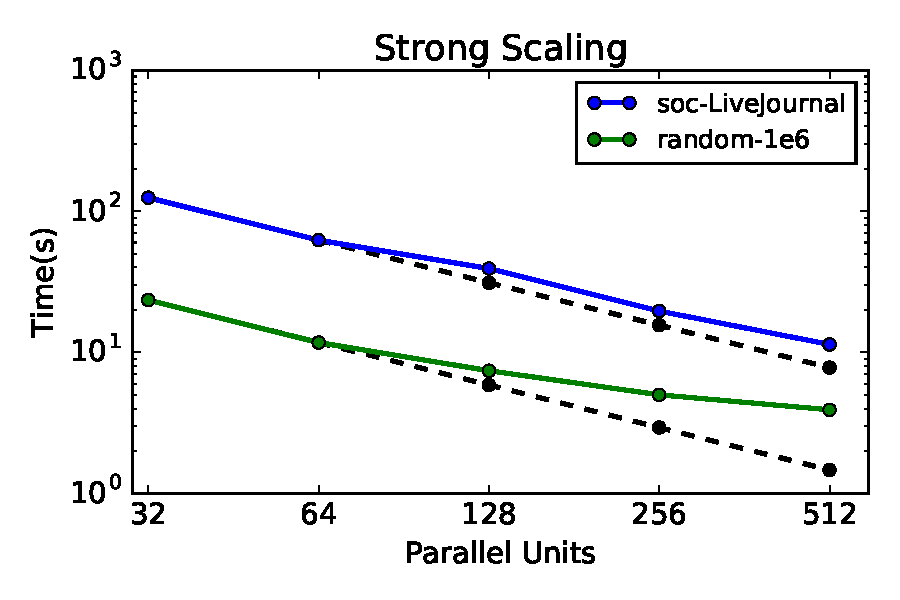
\includegraphics[width=0.45\textwidth]{img/strong-scaling-kpath.pdf}
%     \caption{\label{fig:scale-kpath} k-Path}
%   \end{subfigure}\\
  
%   \begin{subfigure}[b]{\textwidth}
%     \centering
%     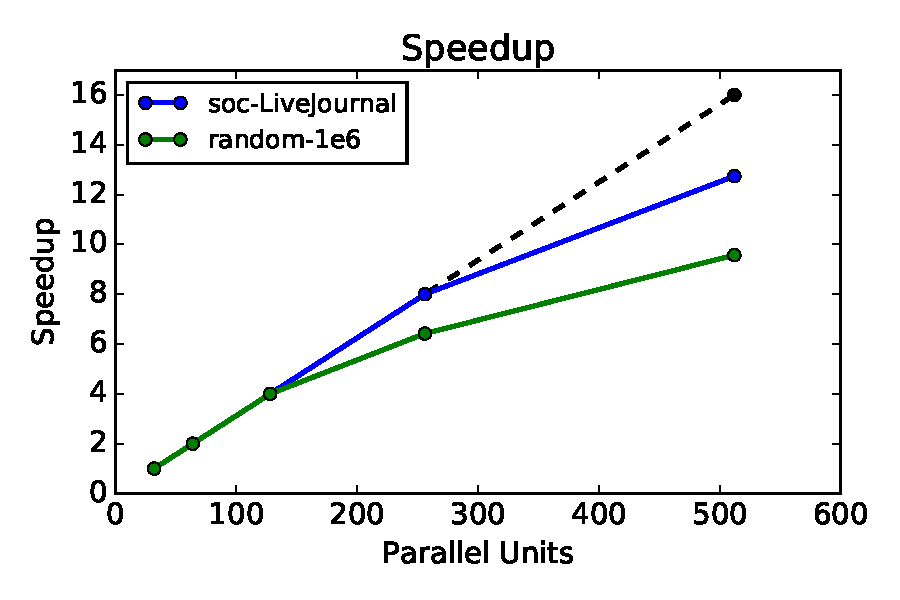
\includegraphics[width=0.45\textwidth]{img/speedup-multilinear.pdf}
%     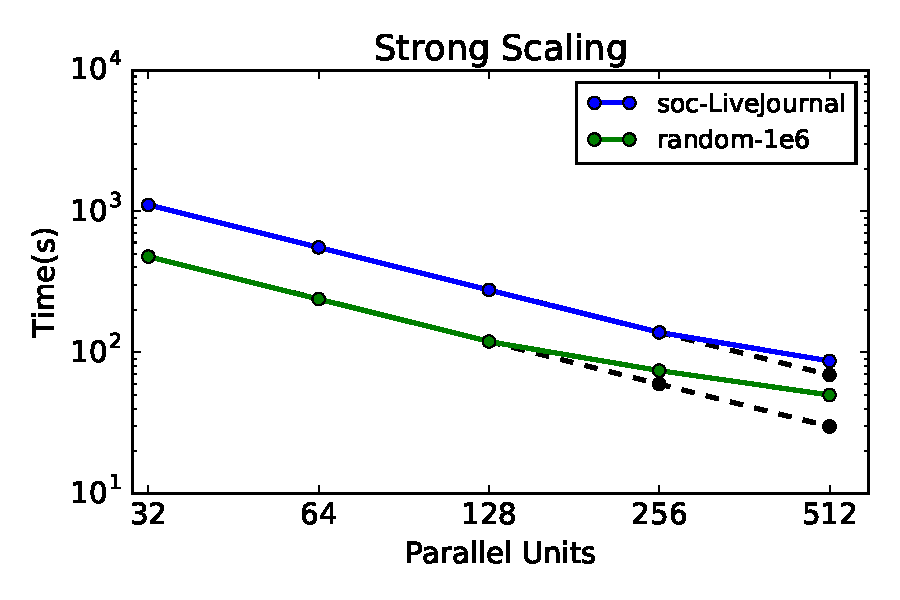
\includegraphics[width=0.45\textwidth]{img/strong-scaling-multilinear.pdf}
%     \caption{\label{fig:scale-multilinear} Multilinear Scan}
%   \end{subfigure}%
%   \caption{Speedup and strong scaling of our MPI algorithms for $k$-Path (\ref{fig:scale-kpath}) and Multilinear Scan (\ref{fig:scale-multilinear}).}
%  \label{fig:scaling}
% \end{figure*}

% \subsection{Comparision with Giraph}
% \label{sec:compare-giraph}
% %Performance for varying k=1 to k=16 in increments of 2
% %This can include both random-er and snap graphs
% We now compare our \parmaxwt{} with an implementation of Algorithm \ref{alg:multilinear-detect} in Giraph, which is a ``think like a vertex" computation framework. In Figure \ref{fig:giraph-comparison}, we show the running time of \parmaxwt{} and the Giraph implementation as a function of $k$. Giraph uses all the available parallel units for each of the $2^k$ circuit evaluation. Therefore, for a fair comparison, we report the time per iteration of both implementations---even though \parmaxwt{} runs multiple evaluations in parallel. Our MPI algorithm shows much better scalability with $k$, giving as much as 5x speed up  over Giraph in the LiveJournal network. We also implemented a version using Spark's GraphX library, but the communication cost associated with the dataflow model in Spark was prohibitively expensive for this algorithm. Giraph, on the other hand, follows a peer-to-peer communication model, similar to MPI, making it a better choice than GraphX.

% \begin{figure}[!htpb]
% 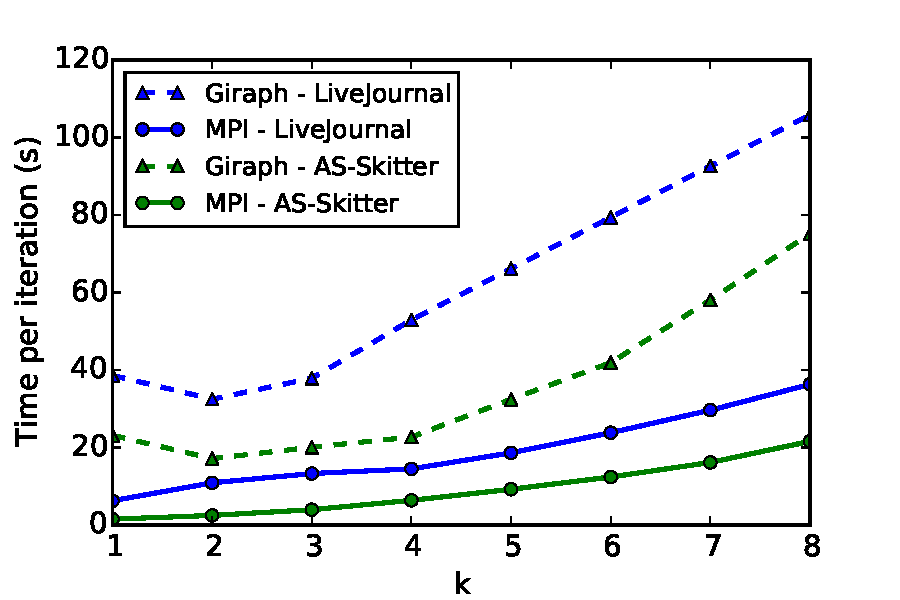
\includegraphics[width=0.4\textwidth]{img/giraph-comparison.pdf}
% \caption{Running time of \parmaxwt{} as a function of $k$ compared to a Giraph implementation.}
% \label{fig:giraph-comparison}
% \end{figure}



% \begin{figure}[!htpb]
% %\frame{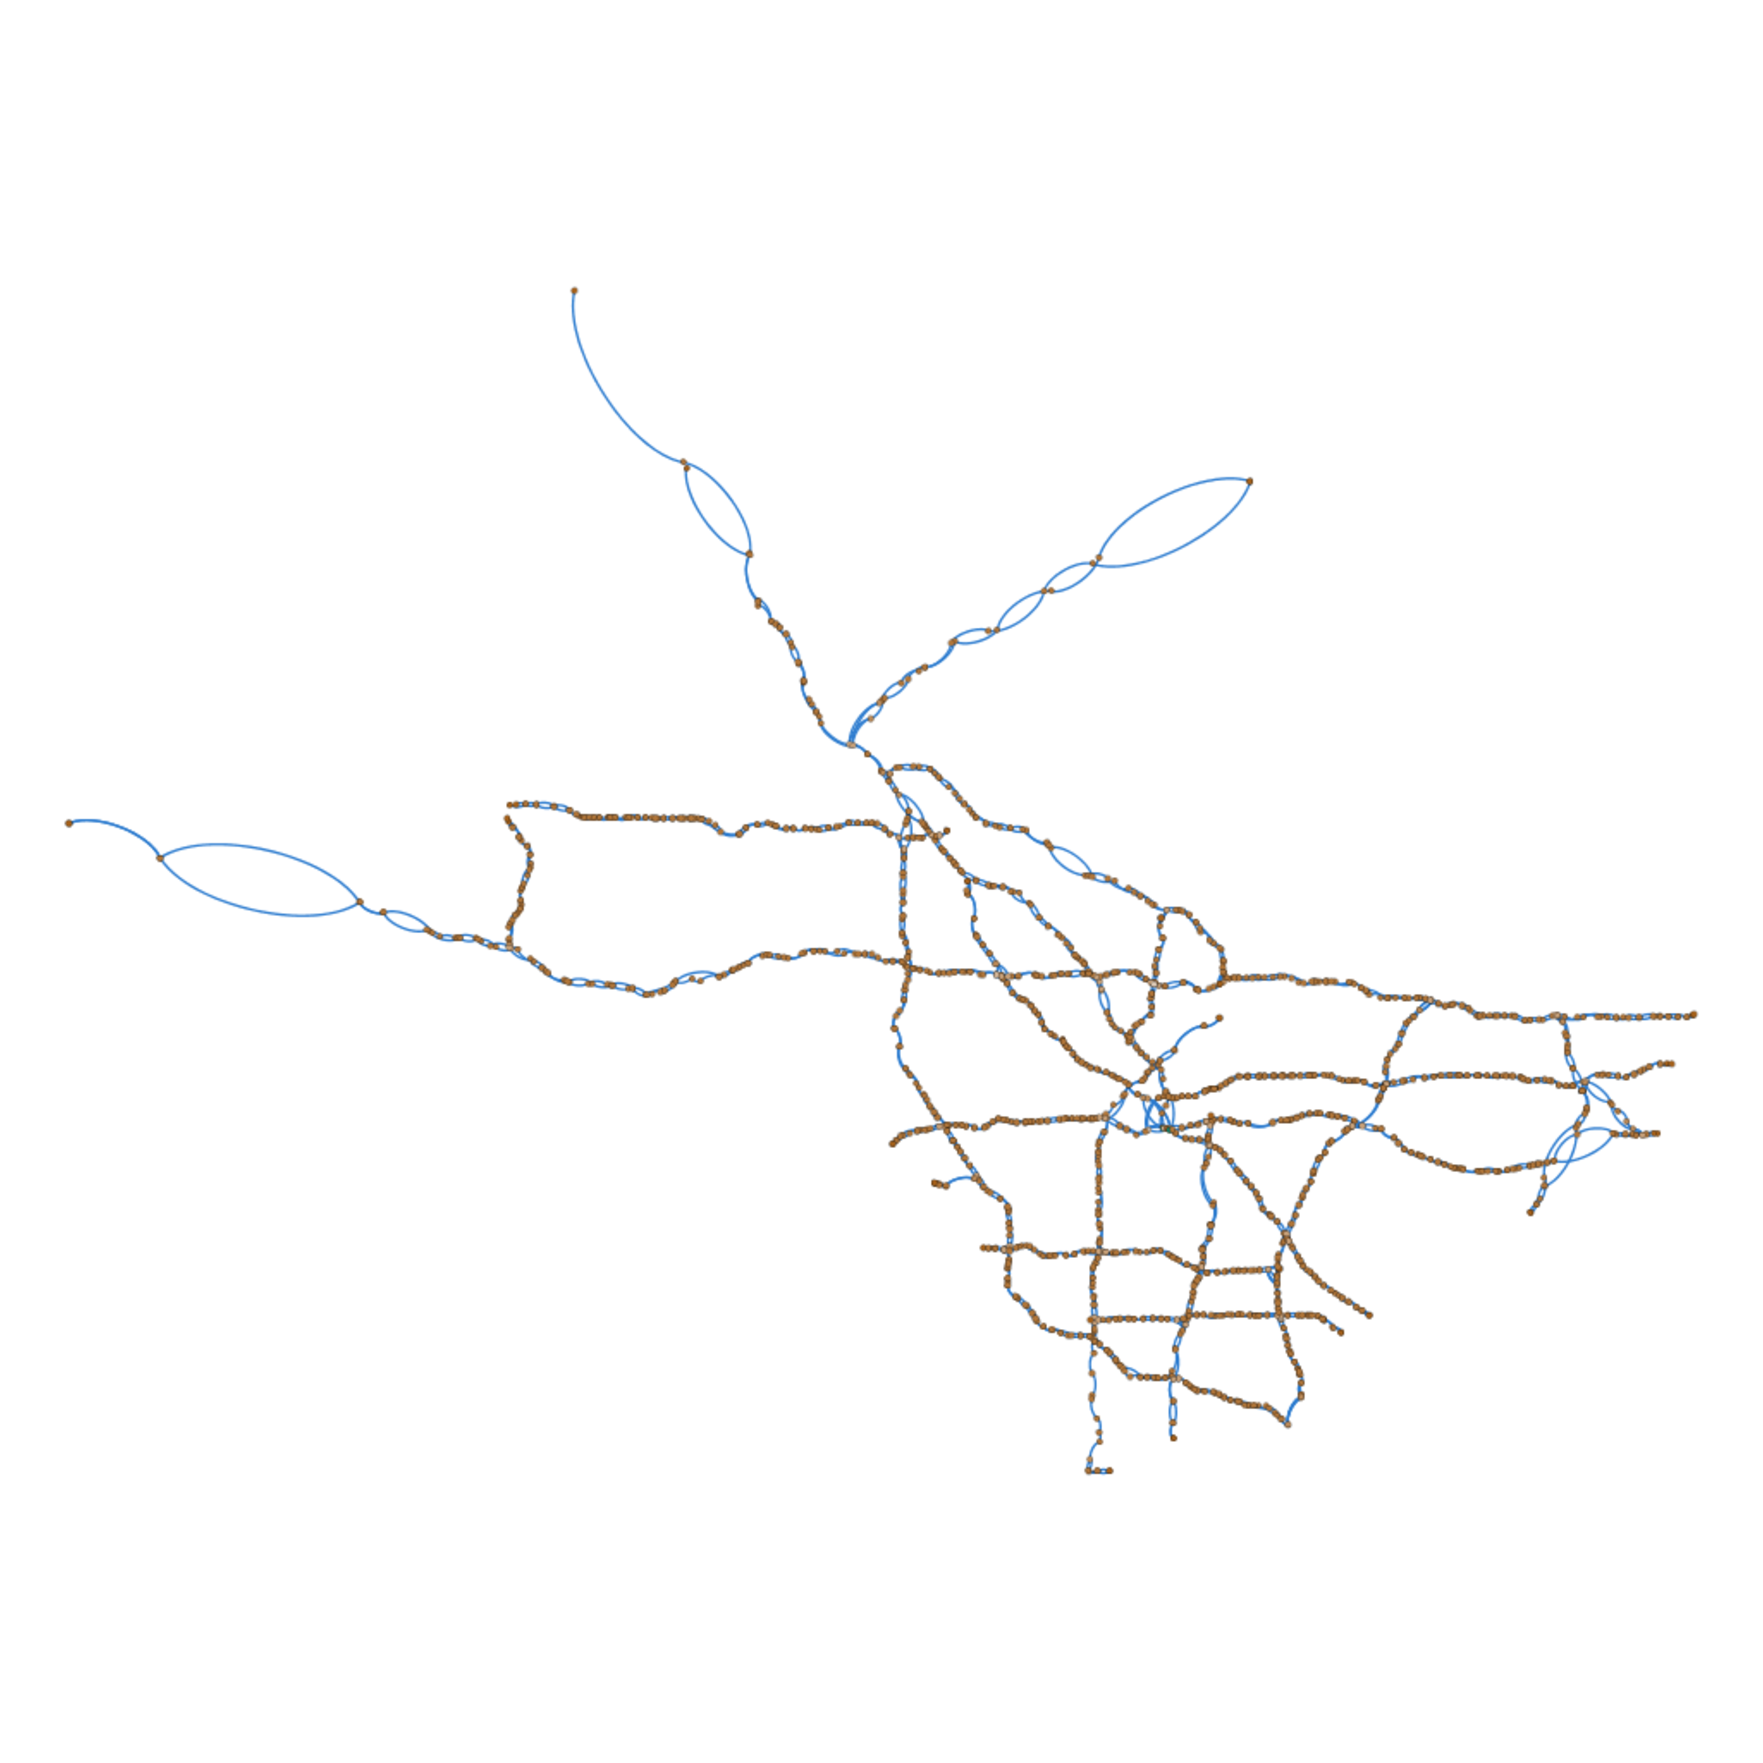
\includegraphics[width=0.48\textwidth,trim={0 4cm 0 4cm},clip]{img/traffic-network.pdf}}
% 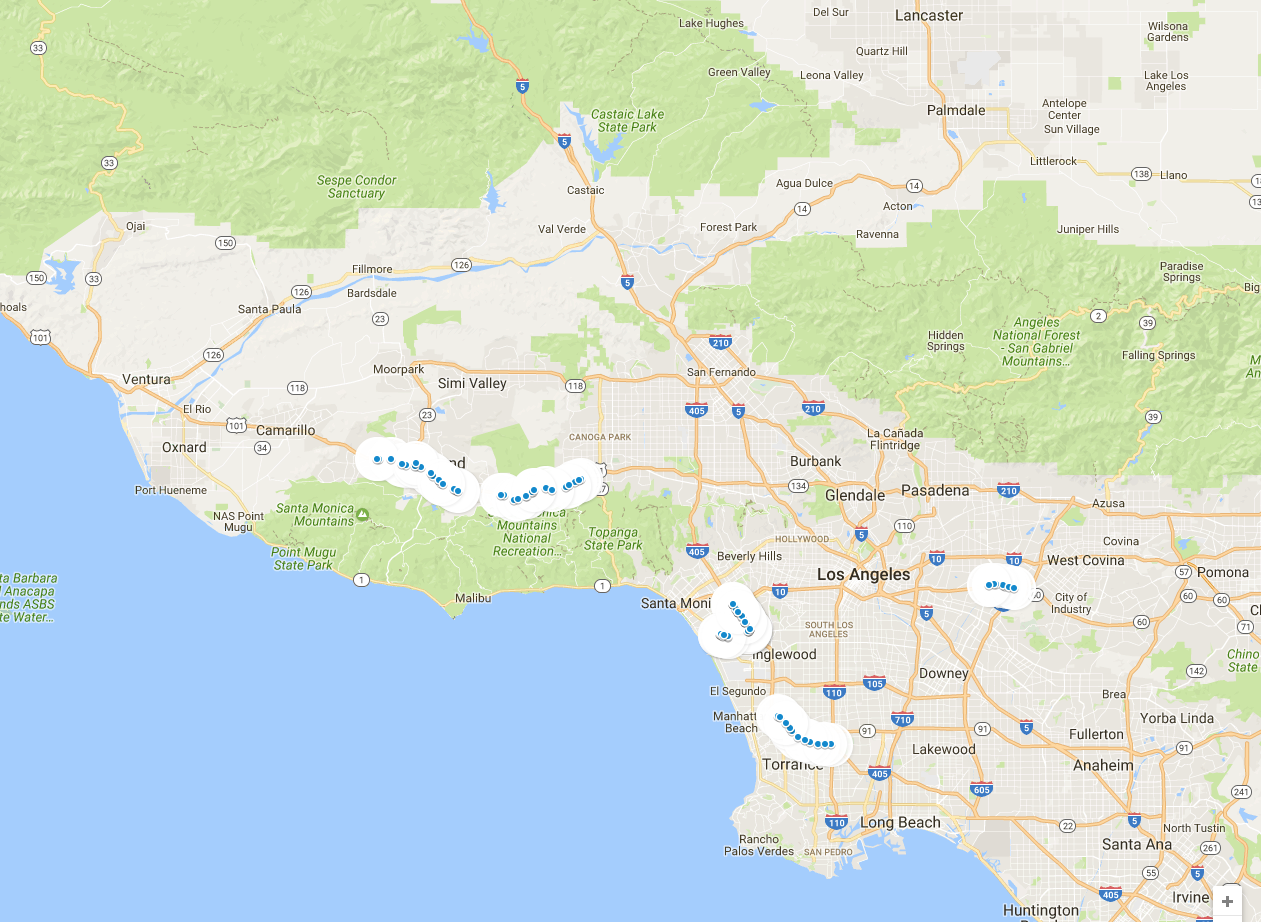
\includegraphics[width=0.48\textwidth]{img/traffic-example.png}
% \caption{Discovering highway segments with unexpected congesion in the Los Angeles road network.}
% \label{fig:traffic}
% \end{figure}


